MongoDB Compass ist eine grafische Oberfläche für MongoDB. Es ermöglicht dem Nutzer, die gespeicherten Daten in der Datenbank grafisch zu analysieren und ohne MongoDB Kenntnisse abzufragen. MongoDB Compass kann außerdem verwendet werden, um die Leistung zu optimieren und Indizes zu verwalten.\newline

MongoDB Compass ist eine intuitiv bedienbare und leistungsstarke Benutzeroberfläche zur Verwaltung von MongoDB-Datenbanken. Sowohl Entwickler:innen als auch Datenbankadministrator:innen können davon profitieren, da sie Datenbanken entwerfen, überwachen und analysieren können, ohne direkt mit der MongoDB-Shell interagieren zu müssen. 
\cite{mongo_compass}

\begin{figure}[h!]
    \centering
    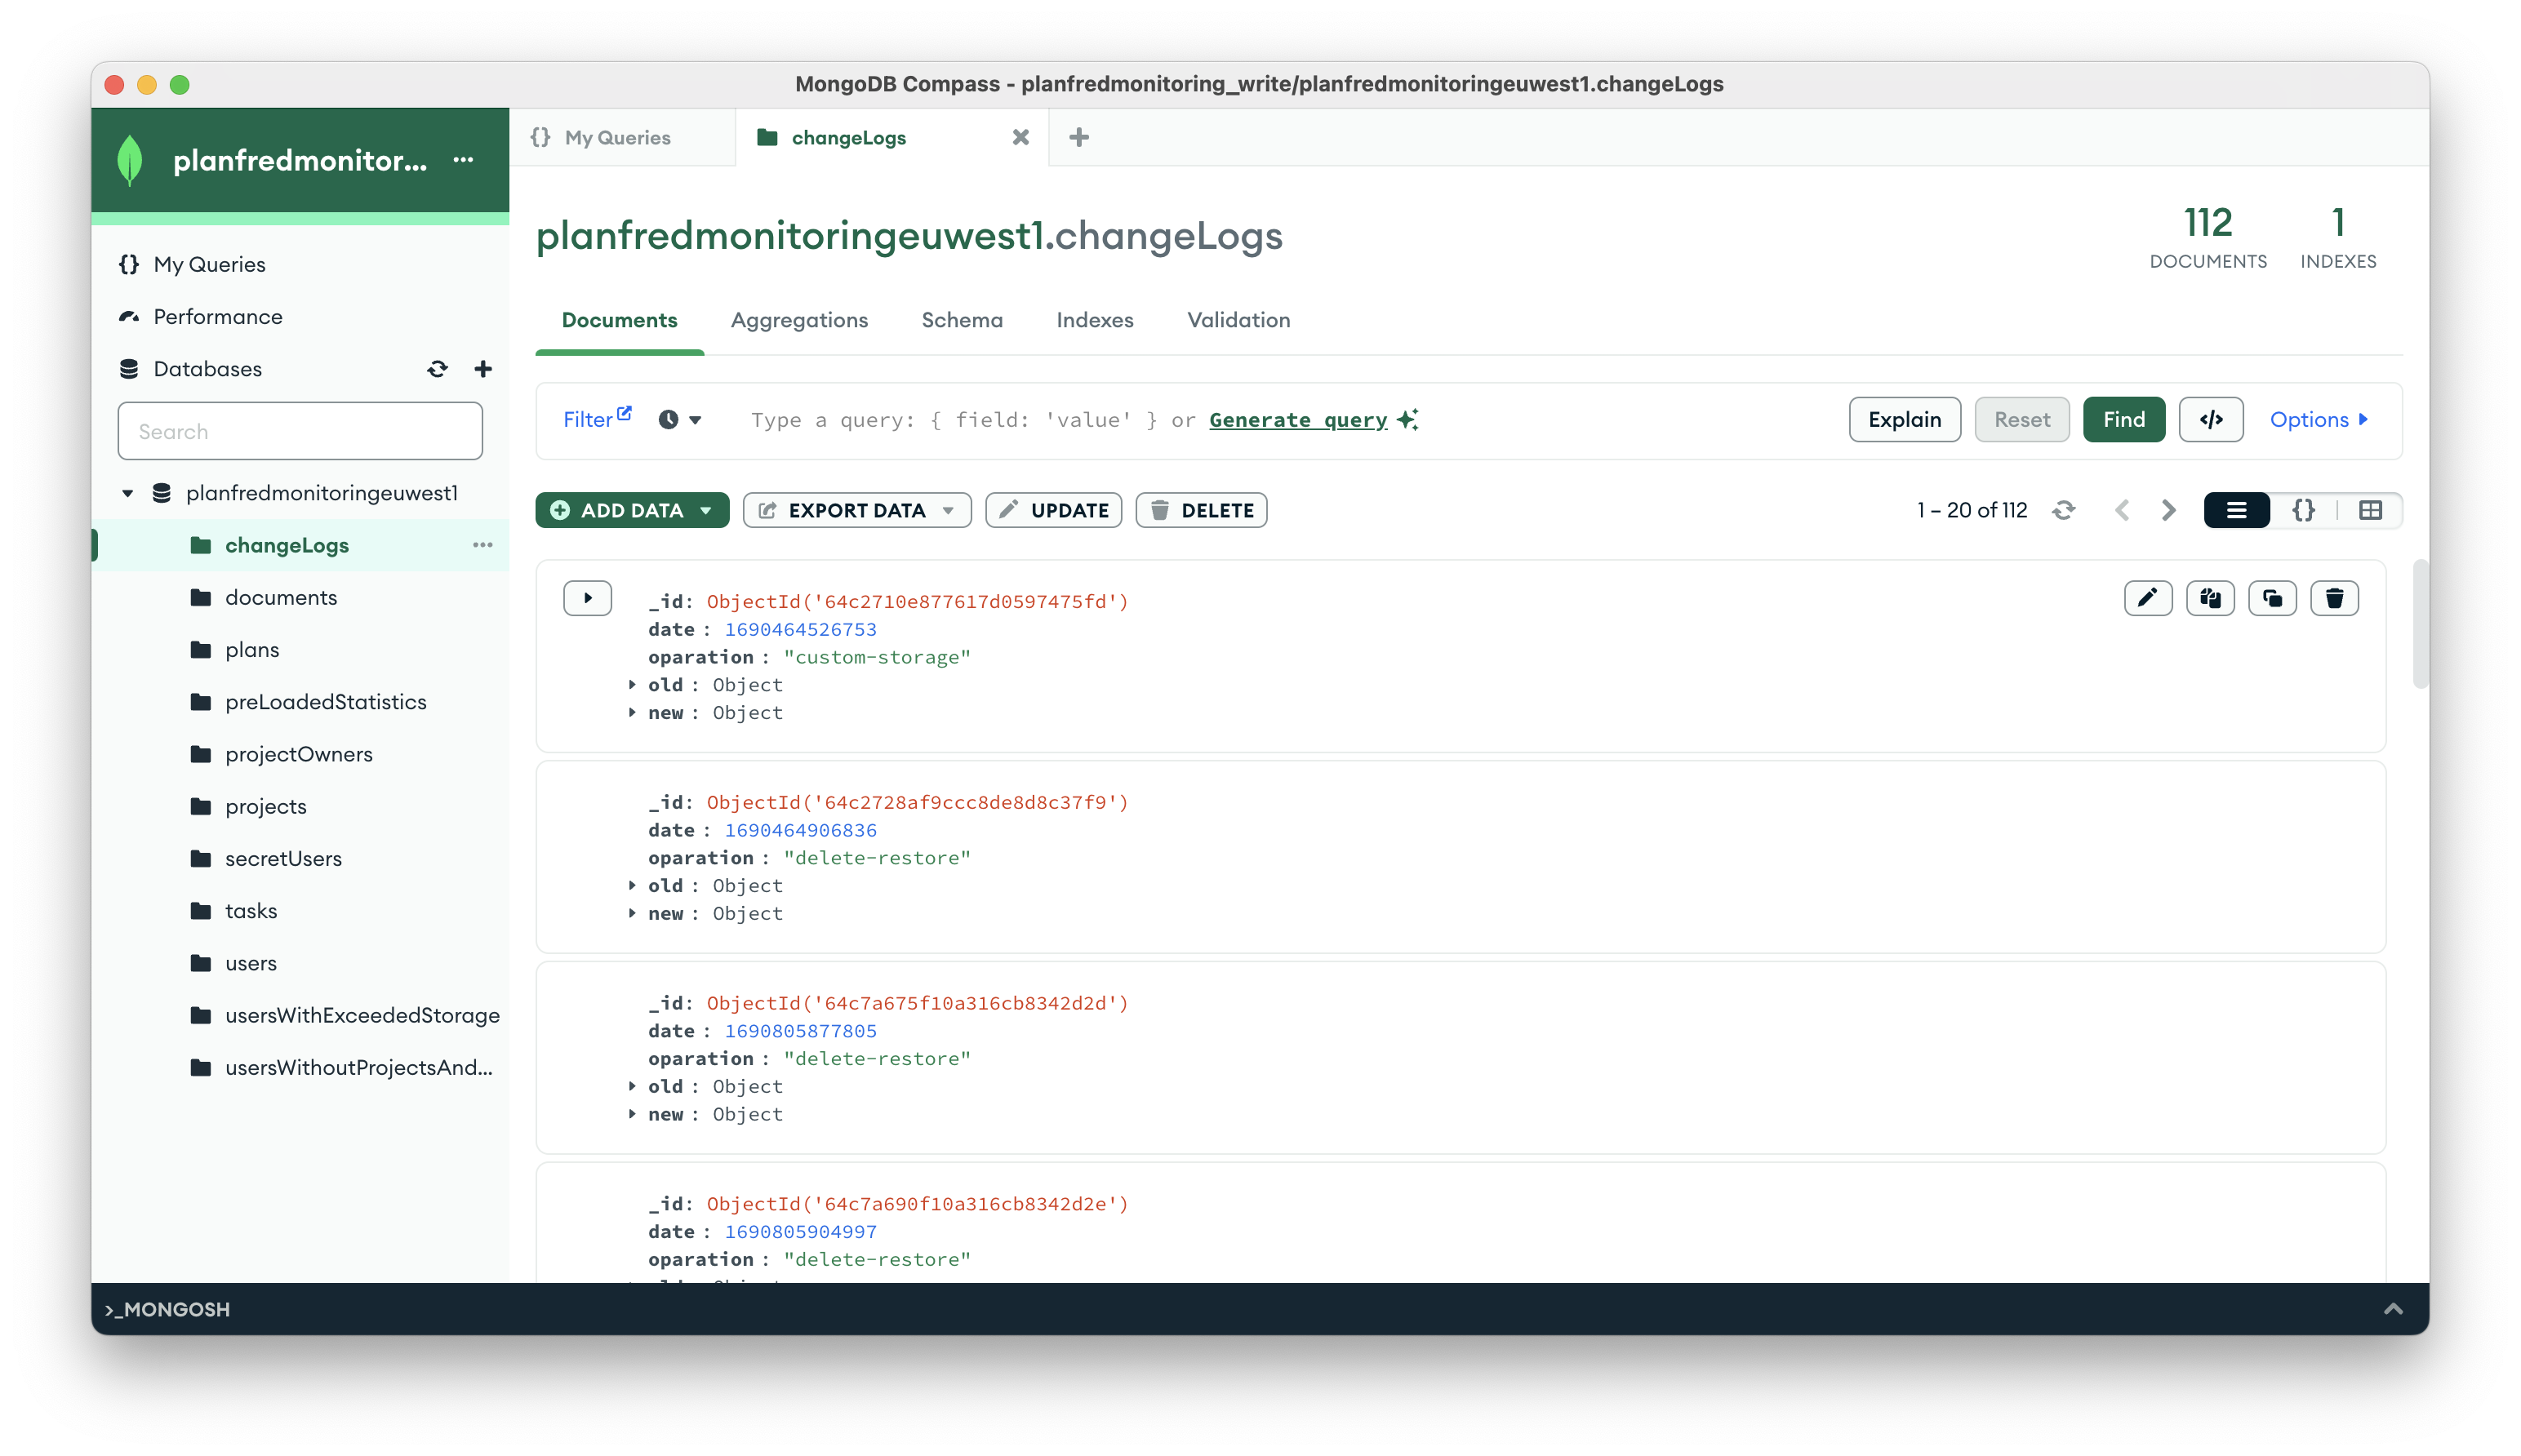
\includegraphics[width=1\linewidth]{pics/mongodb-compass.png}
    \caption{MongoDB Compass}
    \label{fig:enter-label}
\end{figure}

